
\chapter{Enfoque y Herramientas\label{chap:Enfoque-y-Herramientas}}

En este capítulo se describe el enfoque propuesto para extraer información
y conocimiento de un conjunto de características inherentes a componentes
de software y propiedades estáticas y dinámicas del dispositivo android
de ejecución para analizar las relaciones y dependencias y predecir
atributos no funcionales en base a dichas propiedades. Para el diseño
se hizo énfasis en la optimización combinada de los parámetros de
los algoritmos de aprendizaje automático. 

El enfoque plantea llevar a cabo la predicción de propiedades no-funcionales
mediante un proceso de aprendizaje de máquina a través de \emph{i})
la recolección de indicadores o mediciones tomados a partir de la
información provista de la ejecución de piezas de software, considerando
atributos de componentes, atributos inherentes al problema de entrada,
y atributos de la operación y resultados de la ejecución, y \emph{ii})
la construcción de modelos como un proceso interactivo con el usuario
a partir de la configuración inicial de los datos, la optimización
automática de los parámetros de acuerdo a las tasas de error arrojadas
por métricas de evaluación y el ajuste final del modelo a través del
análisis de las curvas de aprendizaje. 

Como soporte para el enfoque, se desarrollaron dos herramientas independientes
entre sí y diseñadas para efectuar el objetivo y conexión de las dos
fases propuestas. Por un lado, se desarrolló una herramienta denominada
\emph{Android Performance Testing and Prediction} cuyo diseño se adapta
fácilmente a la implementación de cualquier dominio computacional
del que se quiera obtener indicadores de desempeño. Al tratarse de
un framework implementado para el sistema Android, permite obtener
de manera directa los benchmarks del dispositivo de interés para el
análisis. Por otro lado, se desarrolló una herramienta standalone
denominada \emph{Nekonata} diseñada para brindar soporte al uso de
las funciones de cualquier librería que realice aprendizaje automático
y minería de datos escritas en lenguaje Java y que consiste en dos
fases, una primer etapa para la construcción del modelo a partir del
conjunto fuente de benchmarks mediante un proceso de automatización
de los algoritmos en complemento de información gráfica para la colaboración
interactiva del usuario y finalmente una segunda etapa de ajustes
al modelo teniendo en cuenta los efectos de overfitting y underfitting
consecuentes del entrenamiento. 

Estas cuestiones se describen en detalle de la siguiente manera. En
la sección \ref{sec:Aplicaciones-de-la} se enumeran algunos de los
usos prácticos de los modelos incluyendo aplicaciones de la propuesta.
Luego, en la sección \ref{sec:Etapas-del-m=0000E9todo} se profundiza
sobre las distintas etapas del enfoque y flujo de trabajo. En la sección
\ref{sec:Herramientas} se describen cada uno de los frameworks desarrollados,
presentando la herramienta para la recolección de datos en la subsección
\ref{subsec:Framework-de-medici=0000F3n} y finalmente, en la sección
\ref{subsec:Herramienta-de-entrenamiento} se presenta la herramienta
para la construcción de modelos evaluativos. 


\section{Aplicaciones de la propuesta \label{sec:Aplicaciones-de-la}}

Los problemas de clase NP - Completos están presentes en la mayoría
de ámbitos computacionales. Afortunadamente, en la medida que estos
problemas resultan difíciles de resolver frente a los peores casos
de entrada, se hace más factible resolverlos aún considerando problemas
de grandes instancias. 

Desafortunadamente, estos algoritmos pueden exhibir variaciones extremas
de ejecución a través de las instancias con distribuciones reales,
incluso, aunque la dimensión del problema se mantuviera constante,
la misma instancia puede requerir dramáticamente diferentes tiempos
de ejecución en función del algoritmo utilizado. Existe una escasa
comprensión teórica de las causas de esta variación. Durante la última
década, una cantidad considerable de trabajo ha intentado demostrar
cómo utilizar las técnicas de aprendizaje automático supervisado para
la construcción de modelos de regresión que proporcionen respuestas
aproximadas a esta pregunta en base a los datos de rendimiento del
algoritmo analizado, en otras palabras, podría creerse que es posible
predecir el tiempo que requerirá un determinado algoritmo para ejecutarse
bajo una entrada en particular construyendo un modelo de tiempo de
ejecución del algoritmo como una función de las características específicas
de cada instancia del problema. 

La construcción de tales modelos conocidos como \emph{modelos de actuación
empírica }(EPM por sus siglas en inglés) ha ido creciendo y motivada
debido a la utilidad que presentan frente a una gran variedad de contextos
prácticos. A continuación, se detallan algunos:
\begin{description}
\item [{Selección~de~algoritmos}] Como se ha tratado en algunos trabajos
\citet{Hutter2014}, los modelos de predicción son útiles para la
selección automática de algoritmos y la configuración en una variedad
de formas (un problema clásico de selección del mejor algoritmo entre
un determinado conjunto); a través de \ac{EPM} se logra predecir
el rendimiento de cada uno de estos algoritmos candidatos y mediante
un análisis comparativo, seleccionar el más apropiado considerando
la instancia del problema y las características del hardware. 
\item [{Ajustes~de~parámetros~y~configuración~automática~del~algoritmo}] \ac{EPM}
sirve a dos propósitos fundamentales, por un lado, modelar el comportamiento
o funcionalidad de un algoritmo parametrizado en base a la configuración
de tales parámetros, en cuyo caso se puede alternar entre el aprendizaje
del modelo y su uso para identificar configuraciones interesantes
para evaluar posteriormente. Por otro lado, se puede modelar el rendimiento
del algoritmo basado conjuntamente en las características de las instancias
del problema y la configuración de sus parámetros. Tales modelos pueden
utilizarse para ajustar los valores de tales parámetros y obtener
una mejor predicción basada en la instancia particular. 
\item [{Generación~de~benchmarks~fuertes}] Un modelo predictivo para
uno o más algoritmos se puede utilizar para establecer los parámetros
de los generadores de benchmarks existentes con el fin de crear instancias
asociadas al algoritmo particular. 
\item [{Obtener~una~visión~general~de~las~instancias~y~el~rendimiento~de~los~algoritmos}] \ac{EPM}
se puede utilizar para evaluar las características de la instancia
y los valores de los parámetros del algoritmo que más impactan en
el rendimiento. Algunos modelos son compatibles con este tipo de evaluaciones
directamente. Para otros modelos, existen métodos de selección de
atributos (características genéricas) para identificar un grupo más
reducido de entradas del modelo que son claves, y describen el rendimiento
del algoritmo casi tan bien como todo el conjunto de entradas. 
\item [{Selección~de~Servicio~y~composición}] Cuando varios servicios
web implementan la misma funcionalidad, los modelos de rendimiento
resultan ser un buen criterio para escoger el mejor candidato entre
ellos. Incluso en tiempo de ejecución, los proveedores de servicio
pueden cambiarse si las condiciones del contexto y los parámetros
de entrada se modifican. 
\item [{Programación~de~tareas~en~redes~móviles}] Suponiendo un conjunto
de tareas que deben asignarse entre un conjunto de dispositivos, los
modelos de rendimiento podrían obtener una medida exacta del tiempo
de respuesta que cada tarea requerirá sobre cada dispositivo con el
fin de minimizar el tiempo total de secuenciación de las tareas. 
\item [{Otros.}]~
\end{description}

\section{Etapas del método\label{sec:Etapas-del-m=0000E9todo}}

El enfoque propuesto se conceptualiza como un proceso de tres fases
complementarias. Este ciclo o flujo de trabajo da lugar a tres etapas
bien definidas por cada dominio o escenario de estudio, desde la obtención
de indicadores hasta la predicción de propiedades no funcionales en
entornos de aplicación. La figura \ref{fig:method-stages} muestra
un esquema conceptual del enfoque, cuyas etapas se describen a continuación:

\begin{figure}
\begin{centering}
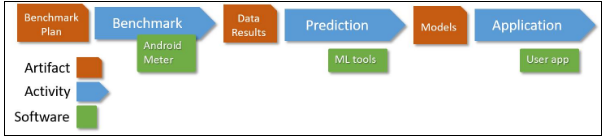
\includegraphics[scale=0.55]{C:/Users/usuario/Tesisworkspace/Tesis_Standalone/tesis/images/method-stages}
\par\end{centering}

\caption{Esquema conceptual del enfoque en fases. \label{fig:method-stages}}
\end{figure}



\subsection{Etapa recolección de datos }

\noindent El proceso comienza con la creación de datasets. Cada dataset
pertenece a un escenario o dominio diferente, del cual se extraen
todas las características que podrían influir sobre el desempeño del
componente. Durante la ejecución de cada servicio o pieza de software
se van realizando las mediciones o métricas sobre distintos aspectos
de la operación y registrando cada uno de estos benchmarks en un archivo
para su posterior análisis. A su vez, el proceso de recolección de
benckmarks involucra la ejecución de sub etapas, pudiendo requerir
el proceso algunas, o todas de las tareas que se detallan a continuación:
\begin{itemize}
\item Integración de componentes: A menudo se requiere la evaluación de
componentes de terceros, tanto de servicios Web como librerías instaladas,
de manera que deben ser integrados correctamente a la herramienta
para ser tratados como componentes. 
\item Selección de características del contexto: Mientras se realiza la
ejecución de los componentes, las propiedades no funcionales del dispositivo
móvil donde se llevan a cabo las operaciones, pueden ser capturadas
como indicadores. Realizar las mediciones en distintos modelos de
dispositivos móviles persigue la idea sobre la influencia de las capacidades
de cada modelo en las operaciones de ejecución. Ya que las predicciones
son realizadas sobre componentes de aplicaciones Android, la captura
de las carecterísticas estáticas y dinámicas son tomadas en cuenta,
para detectar relaciones entre éstas y los atributos a predecir de
los componentes.
\item Implementación de dominios: La evaluación de casos de estudios variables
en complejidad y características,que incluyen diferentes formatos
de componentes, son analizados con el fin de arrojar conclusiones
sobre la variación en el desempeño de las técnicas de regresión frente
a diferentes ambientes, analizar la calidad en el aprendizaje para
atributos no funcionales; cuánta mejora en la precisión significa
la aplicación de técnicas de regresión sobre problemas de complejidad
polinómica respecto a problemas NP, o la afectación en el tiempo de
respuesta de las operaciones sobre servicios remotos frente a servicios
locales, son algunas de las conclusiones que podrían desprenderse
del análisis. 
\item Generación de instancias de entrada: Se debe proveer una manera para
generar arbitrariamente instancias de un dominio particular, o la
capacidad para obtener instancias externamente a través de enlaces
o archivos. 
\item Selección de características de la entrada: Es posible obtener atributos
propios a la entrada del dominio, generalmente atributos que configuran
o sirven para generar una instancia. 
\item Ejecución de componentes y obtención de métricas: Los componentes
son ejecutados con las entradas generadas, tomando y registrando mediciones
sobre las características incorporadas además de las propiedades de
interés a predecir. De esta forma, los dataset pueden ser formados
por una cantidad variable y opcional de atributos en base a las características
que hayan sido elegidas para ser medidas. Este factor impacta en la
calidad del dataset creado, por lo tanto estudiar el comportamiento
que adoptan los datos y la distribución en el rango de valores, puede
servir de indicio para entender el desempeño de las técnicas. 
\end{itemize}

\subsection{Etapa aprendizaje}

A partir del conjunto de benchmarks obtenidos en la etapa anterior,
se aplican técnicas de aprendizaje de máquina para la extracción de
conocimiento de los datos. Tal conocimiento se refleja mediante la
construcción de modelos predictivos que mejor se ajustan a la generalización
de la información mediante un proceso de entrenamiento, optimización
y evaluación de los mismos. El proceso de aprendizaje requiere indefectiblemente
de un conjunto de datos de entrenamiento volcado en un archivo, un
atributo de ese conjunto a predecir y un conjunto de algoritmos que
aplican técnicas de regresión sobre los datos. Actualmente, hay herramientas
que proveen estos algoritmos incluyendo toda la funcionalidad necesaria
para este proceso, y que son fácilmente integrables a cualquier desarrollo.
Además, el aprendizaje está conformado por varias etapas o sub procesos.


\paragraph{Configuración de las técnicas }

Las técnicas de regresión representan modelos matemáticos cuyas funciones
involucran diferentes parámetros de configuración. La variabilidad
en estos valores permite ajustar las preferencias del algoritmo y
consecuentemente, la obtención de modelos de calidad diferente. Por
lo tanto, el desafío principal de esta parte de la etapa es encontrar
los valores apropiados para cada uno de los parámetros, teniendo como
base, el conocimiento sobre el efecto que el parámetro causa en el
algoritmo. Al obtener la mejor configuración de una técnica, para
un dataset y un atributo particular, se facilita la comparación simultánea
de todas las técnicas disponibles a través de las métricas de evaluación
y en consecuencia seleccionar la más óptima. 




\paragraph{Construcción de modelos }

La construcción de modelos predictivos es un proceso que inicia con
el entrenamiento de los datos, continúa opcionalmente con un proceso
de validación y concluye con una evaluación del error cometido en
las estimaciones frente a los datos reales del entrenamiento.

La implementación de los casos de estudio enfatizan la predicción
de la precisión en las respuestas y el tiempo de ejecución de los
componentes considerando a ambas métricas esenciales al momento de
seleccionar el/los componente/s más adecuado/s para un propósito particular,
dadas ciertas entradas, componentes posibles, restricciones y parámetros
deseados.

La fase de entrenamiento de este proceso utiliza las mediciones ya
obtenidas en la etapa anterior y a partir del atributo que se desea
predecir, el algoritmo va definiendo la función de regresión para
encontrar las relaciones entre los atributos del dataset y el atributo
a predecir. Esta fase concentra el mayor porcentaje del tiempo computacional
y uso de memoria, y varía de acuerdo a la complejidad o simplicidad
de cada técnica en particular. 


\paragraph{Evaluación de modelos}

Una vez concluida la fase de entrenamiento, la calidad del modelo
obtenido debe ser analizada para determinar la medida en que el modelo
será capaz de generalizar cualquier entrada de dataset futura. La
noción sobre el desempeño del modelo tiene lugar a partir de métricas
ya definidas para modelos de regresión, que capturan distintamente
el error de predicción e incluyen el coeficiente de correlación para
conocer el grado de interdependencia de las variables. 

A pesar que el objetivo de alcanzar estimaciones bajas en error es
importante, el análisis no debe centralizarse únicamente en la minimizacíón
del error en las predicciones, sino que debe estar dirigido por las
curvas de aprendizaje. Las curvas de aprendizaje permiten observar
gráficamente el modo en que el modelo se ajusta a los datos de entrenamiento,
evidenciando efectos de sobreajuste, el modelo sólo será bueno para
ese dataset en particular, o efectos de baja adaptación, debido principalmente
a que no se cuenta con los suficientes datos para enseñar al modelo. 


\subsection{Etapa predicción }

Finalmente, se pretende utilizar estos modelos de predicción en entornos
de aplicación que permitan la selección del componente más adecuado
en base a un conjunto de propiedades del problema de entrada, las
propiedades internas del dispositivo en el cual se llevará a cabo
la ejecución, y un conjunto de restricciones que deben satisfacerse,
a través de un proceso automatizado que determine al usuario la opción
más favorable evitando la ejecución individual de cada componente. 


\section{Herramientas\label{sec:Herramientas}}

El trabajo presentado conforma dos de las tres fases propuestas para
el enfoque global del desarrollo. La primer fase se lleva a cabo en
un framework particular para la medición de propiedades de componentes
Android que será detallada en la sección \ref{subsec:Framework-de-medici=0000F3n}.
La segunda fase para la construcción de modelos predictivos a través
de técnicas de aprendizaje de máquina se desarrolla en una segunda
herramienta la cual será detallada en la sección \ref{subsec:Herramienta-de-entrenamiento}. 


\subsection{Framework de medición para Android\label{subsec:Framework-de-medici=0000F3n}}


\subsubsection*{Enfoque general}

\emph{Android Performance Testing and Prediction} es un framework
diseñado para realizar mediciones de performance de componentes ejecutados
bajo el sistema Android. Es una herramienta de testing que permite
ejecutar diferentes piezas de software y evaluar propiedades influyentes
y características del entorno de ejecución. 

La herramienta cuenta con el soporte necesario para adaptarse a cualquier
dominio informático y exportar las mediciones correspondientes en
archivos de formato \ac{CSV}, mediciones que servirán de fuente para
herramientas de predicción a través de técnicas de aprendizaje de
máquina. 


\subsubsection*{Objetivos}

El rendimiento de los componentes de ejecución (algoritmos, servicios
Web, procesos ejecutándose en segundo plano, etc.) dependen de varios
factores: el contexto de ejecución donde el componente está funcionando,
los parámetros de entrada que requiere el componente de la operación
y su implementación interna. Sin embargo, al utilizar componentes
de terceros es posible desconocer el modo en el que fueron implementados,
actuando como cajas negras a los desarrolladores móviles, que sólo
conocen sus interfaces de aplicaciones, pero no su trabajo interno. 

Para elaborar un análisis del rendimiento, técnicas de aprendizaje
automático sobre los datos recogidos empíricamente pueden ser utilizados
para construir modelos de predicción del tiempo de ejecución del componente,
como una función de los parámetros de entrada y las características
específicas del contexto de ejecución: configuración de algoritmos,
selección de servicios, planificación de trabajos, por citar algunos
ejemplos. 


\subsubsection*{Enfoque}

El enfoque principal de esta herramienta está centrado en dos propiedades:
el tiempo de respuesta y la precisión de los resultados. 

El tiempo de respuesta refiere al tiempo total que demanda un componente
en ejecutar una operación o tarea, es decir, el tiempo para responder
a una solicitud con una entrada determinada. Por otro lado, la precisión
es una medida que evalúa la calidad de los resultados o salida de
un componente y tiene diferentes significados semánticos dependiendo
de la funcionalidad requerida, por ejemplo, en problemas de clasificación,
se toma el concepto de precisión como la medida estadística de la
eficacia de un clasificador, la precisión está relacionada a la identificación
o exclusión correctamente de una condición. En problemas de optimización,
también conocido como optimalidad, la precisión es una relación entre
la solución de salida obtenida y la solución óptima conocida. 

Para construir un modelo de predicción del tiempo de respuesta sobre
un componente particular, se deben considerar dos variables al momento
de evaluar, un conjunto acerca de las características del contexto
de ejecución, por ejemplo, núcleos de CPU, tipo de red, etc. y otro
conjunto acerca de las características de la entrada en particular,
por ejemplo, en tamaño expresado en bytes. 

Del mismo modo se construye un modelo de predicción de precisión sobre
un componente, como en la mayoría de los casos esta medida no depende
de las características del contexto en el que se ejecuta, el modelo
respondería a una función dependiente de las entradas del problema.


\subsubsection*{Componentes}

El análisis de rendimiento que se propone en esta herramienta se basa
en entidades de software individuales de ejecución que proveen servicios
a través de una interfaz específica. De aquí en más, estas entidades
se denotarán componentes. 

\begin{figure}
\begin{centering}
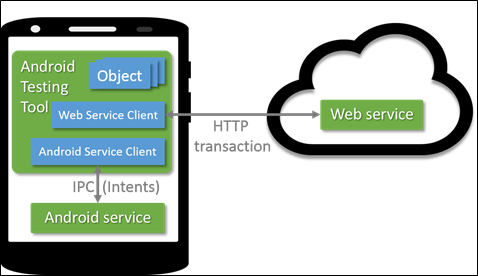
\includegraphics[scale=0.55]{C:/Users/usuario/Tesisworkspace/Tesis_Standalone/tesis/images/android-component}
\par\end{centering}

\caption{Esquema conceptual de componentes Android considerados. \label{fig:android-component}}
\end{figure}


En la figura \ref{fig:android-component} se pueden observar los tres
tipos de componentes generalizados por la herramienta para obtener
los resultados de mediciones adecuados, incluyendo servicios Web y
servicios específicos de la plataforma Android, mientras que para
toda pieza de software remanente los componentes son tratados simplemente
como objetos Java. Las instancias de objetos hacen referencia a cualquier
componente residente en el espacio de memoria de una aplicación, el
componente específico para servicios web incluye cualquier componente
remoto fuera del dispositivo y accedidos a través de protocolos de
comunicación Web, como \ac{HTTP}. Por último el componente específico
para servicios Android incluye cualquier proceso ejecutado en segundo
plano residente en el mismo dispositivo y accedidos a través de objetos
Intent (como único mecanismo de comunicación entre procesos del sistema
Android). 


\subsubsection*{Diseño e implementación}

El proyecto \emph{Android-Testing-Tool} constituye el modelo base
del framework \emph{Android-Performance-Testing-and-Prediction} para
llevar a cabo el proceso de medición de propiedades de cualquier tipo
de componente. Además, se proveen dos proyectos a modo de ejemplo
demostrando el modo de uso de el framework. El proyecto \emph{Evaluation-of-Face-Detection-Services}
fue diseñado para obtener mediciones sobre servicios que ofrecen reconocimiento
facial y el proyecto \emph{Examples-Android-Testing-Tool} fue diseñado
para dominios de problemas NP, incluyendo a problemas de la clase
P y NP - Completos. 

A continuación se expone en la figura \ref{fig:TestingTool-Diagram}
los principales factores que han servido de guía para el diseño del
proyecto base \emph{Android-Testing-Tool}. 

\begin{figure}
\begin{centering}
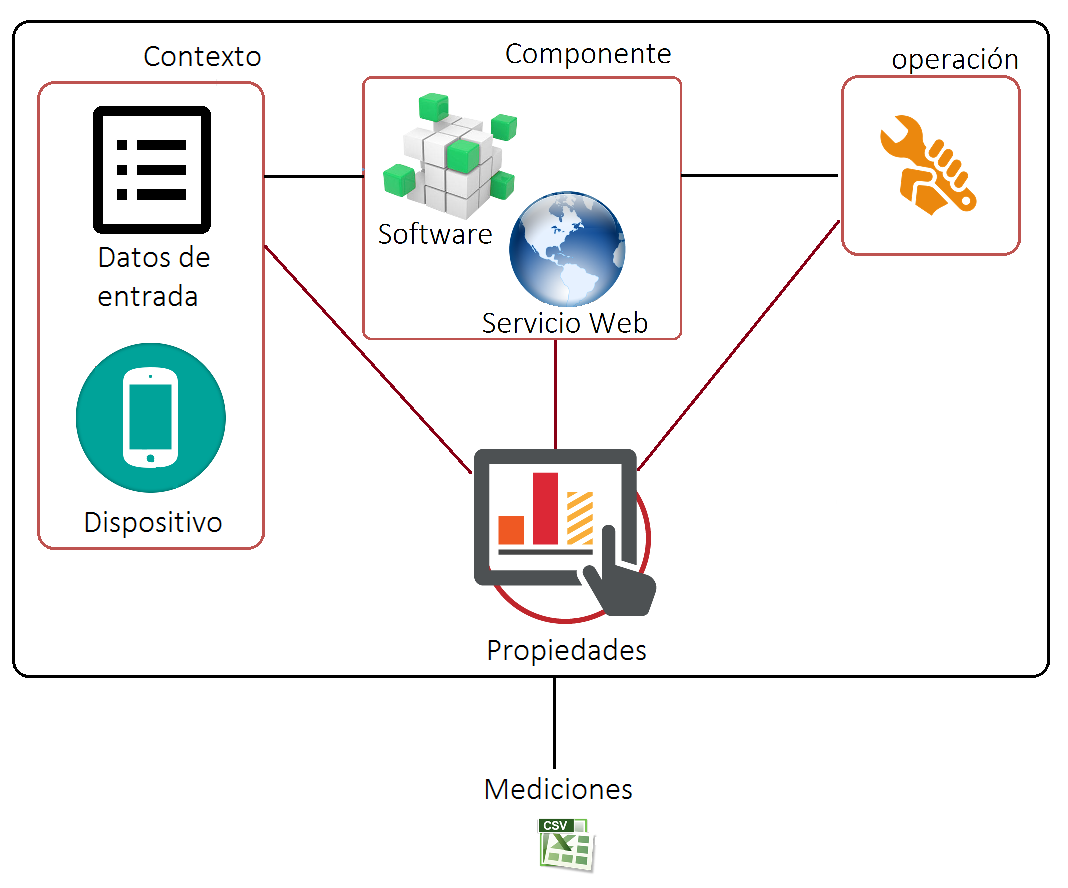
\includegraphics[scale=0.1]{C:/Users/usuario/Tesisworkspace/Tesis_Standalone/tesis/images/TestingTool-Diagram}
\par\end{centering}

\caption{Diagrama estructural de la herramienta template \emph{Android Testing
Tool}.\label{fig:TestingTool-Diagram}}


\selectlanguage{english}%
\selectlanguage{english}%
\end{figure}


La forma de organizar diferentes modelos de evaluación se realiza
a través de la creación de planes de prueba, que se configuran y posteriormente
se ejecutan para obtener un archivo de formato \ac{CSV} con el resultado
de todas las mediciones incorporadas al plan de pruebas. La herramienta
implementa por defecto un objeto llamado \emph{TestPlan} que define
una ejecución sistemática de las operaciones y métricas sobre ellos.
Básicamente, un modelo de plan de pruebas se compone de un conjunto
posible de componentes, un conjunto posible de objetos de entrada,
y un conjunto posible de métricas para realizar las mediciones, dando
la posibilidad de configurar estas propiedades a los requerimientos
deseados. Una vez configurado y ejecutado el plan de pruebas, los
resultados con las mediciones son almacenados en un objeto denominado
\emph{Results} y los datos son exportados a un archivo de formato
\ac{CSV} para su posterior procesamiento. 

La herramienta utiliza una representación simplificada de los componentes,
pudiendo ser éstos servicios Web o simplemente piezas de software
implementadas por el programador. Los parámetros que recibe son dos
objetos del tipo \emph{Input} y \emph{Output}, siendo éstos, instancias
de objetos que representan la entrada y salida del problema respectivamente.
Cada uno de los componentes asociados a un problema específico ejecutan
una operación o tarea a través de la llamada al método \emph{execute}
del componente. Esta operación es responsable de evaluar la ejecución
de la instancia de entrada en el componente y retornar un objeto de
salida o respuesta del problema. Tanto \emph{Input} como \emph{Output}
son dos conceptos abstractos que representan instancias reales del
problema. Una instancia de entrada puede encapsular no sólo los parámetros
requeridos para realizar la ejecución del componente, sino la configuración
de los mismos. Por otro lado, una instancia de salida encapsula la
respuesta o resultado de esa operación. Durante la ejecución del plan
de pruebas (ejecución de cada uno de los componentes asociados), se
evalúan los indicadores que fueron configurados como métricas en el
plan. Se distinguieron cuatro tipos de métricas en función del elemento
de medición, determinando el parámetro que recibe: 
\begin{enumerate}
\item Métricas globales sobre características estáticas del contexto: cualidades
del entorno de ejecución que se mantienen estáticas (sin cambio) durante
el plan de pruebas, por ejemplo, modelo del dispositivo, arquitectura
de la CPU, cantidad de núcleos de CPU, tamaño de memoria, etc. 
\item Métricas generales sobre características de la entrada: atributos
inherentes al dominio del problema, por ejemplo, en el problema de
detección de rostros algunas características podrían ser el nombre
de imagen, tamaño o contraste, formato de archivo, etc.
\item Métricas generales del componente: propiedades del componente como
el nombre, su ubicación, etc.
\item Métricas de operación: Son medidas que actúan sobre la ejecución del
componente, por lo cual distinguen en tres tipos diferentes:

\begin{itemize}
\item Características de la salida: características o métricas obtenidas
a partir del resultado de la operación, por ejemplo el tamaño de la
salida, la precisión de la misma, etc.
\item Características dinámicas del contexto: características del entorno
de ejecución que pueden variar de una operación a otra, como el uso
de CPU, el número de procesos en ejecución, tipo de conexión, ubicación
del dispositivo, etc. 
\item Características de desempeño: medidas de interés sobre el rendimiento
que varían de una operación a otra, como el tiempo de respuesta, el
consumo de batería, operaciones ejecutadas con éxito o con error,
etc.
\end{itemize}
\end{enumerate}
El framework de medición ha sido diseñado para soportar distintos
dominios sobre los cuáles tomar las medidas deseadas. Por el momento
sólo implementa dos tipos de dominios: por un lado, problemas clásicos
del tipo NP para el análisis del desempeño de diferentes algoritmos
de resolución y por otro lado, aplicaciones de propósito general,
en este caso, aplicaciones que ofrecen reconocimiento facial para
la evaluación de diferentes servicios que ofrecen esta misma funcionalidad,
como ya ha sido anticipado. Los problemas de complejidad NP se contemplan
bajo un proyecto individual llamado \emph{Examples-Android-Testing-Tool}
para la evaluación de desempeño de distintos algoritmos considerando
dos aspectos fundamentales: tiempo (aproximación del número de pasos
de ejecución que emplea el algoritmo) y espacio (aproximación de la
cantidad de memoria utilizada). Los problemas implementados pertenecen
tanto a la clase P como a la clase NP-Completos. Por otro lado, el
objetivo de la incorporación de dominios que implican el uso de servicios
remotos se basa en la idea de automatizar el testeo continuo de uno
o varios servicios, en este caso, aplicaciones que ofrecen reconocimiento
facial, teniendo en cuenta las características que estos pueden proveer
y aquellas que el usuario de la aplicación desee considerar, de esta
manera determinar el servicio más adecuado (según el contexto) para
la ejecución de una tarea. Este dominio ha sido diseñado a través
de un proyecto individual bajo el nombre de \emph{Evaluation-of-Faces-Detection-Services}.
Este proyecto se implementó como un modelo básico y genérico sobre
el proceso de detección de rostros. Tal proyecto conforma una estructura
general para almacenar y acceder a todos los atributos posibles que
cualquier servicio que brinde la funcionalidad de detección de rostros
pudiera ofrecer. Es importante destacar algunos detalles sobre los
componentes, entradas y métricas que fueron tomados en cuenta en el
diseño del proyecto. Cada componente representa un servicio particular,
cuya performance es evaluada y analizada; en base a los parámetros
de configuración que acepta cada uno de estos servicios, se generan
diferentes instancias de componentes posibles, un servicio que admite
dos variables de configuración, por ejemplo, da lugar a cuatro tipos
de componentes como producto de la combinación de opciones configurables
posibles. En cuanto a las entradas del dominio, pueden añadirse al
plan de pruebas a través de archivos o de manera estática especificando
la ruta de cada imagen. Finalmente, fueron consideradas métricas respecto
al proceso u operación (rostros correctamente detectados, rostros
detectados y Tiempo de respuesta) y respecto a la imagen de entrada
(contraste, entropía, formato, intensidad promedio, cantidad de rostros
en la imagen, cantidad de pixeles de la imagen, tamaño y nombre).
Respecto al servicio, sólo se registra el nombre del mismo. 


\subsection{Herramienta de entrenamiento y evaluación de modelos\label{subsec:Herramienta-de-entrenamiento}}

El eje que ha guiado el diseño de la herramienta ha sido el brindar
soporte para el uso de cualquier librería que ofrezca aprendizaje
de máquina a través de la implementación de todos los conceptos involucrados
como objetos independientes a los cuales adaptar las funcionalidades
de las librerías. La herramienta \emph{Nekonata} lleva a cabo dos
tipos de procesos en el desarrollo de sus funciones, procesos automatizados
y procesos que requieren la colaboración del usuario con el fin de
mejorar los resultados a partir de vistas gráficas sobre el comportamiento
y características de los modelos y además, para incluir en el proceso
el interés y criterio del usuario. 

El enfoque y objetivo de la herramienta se concluyen en dos etapas,
una fase de entrenamiento de modelos y una fase de evaluación y mejora
de los mismos. 

En la figura \ref{fig:prediction-tool} se muestran las vistas iniciales
de la herramienta , presentación y configuración de datos. 

\begin{figure}
\begin{centering}
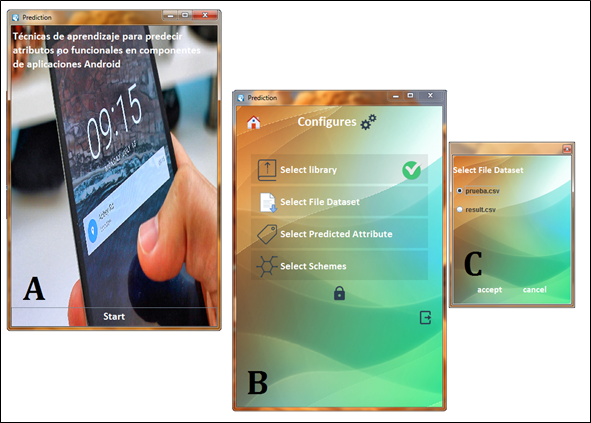
\includegraphics[scale=0.55]{C:/Users/usuario/Tesisworkspace/Tesis_Standalone/tesis/images/prediction-tool}
\par\end{centering}

\caption{Captura de pantalla de la herramienta: (A) Presentación, (B) Configuración
de datos, (C) Menú de selección de opciones.\label{fig:prediction-tool}}
\end{figure}



\subsubsection{Entrenamiento de modelos}

En esta sección se brindará un enfoque global y expresarán las consideraciones
de los conceptos relacionados al proceso de entrenamiento. Posteriormente,
se describe en detalle el flujo de desarrollo del proceso. Estos conceptos
han sido el eje del diseño de la herramienta. A continuación, se presenta
un listado de los objetos tratados: 


\subsubsection*{Librerías}

Al día de hoy se han implementado bibliotecas que realizan aprendizaje
automático en múltiples lenguajes de programación. A pesar de la gran
variación que existe entre unos y otros, el uso de técnicas de aprendizaje
de máquina se rige bajo los mismos conceptos: durante la etapa de
entrenamiento, un conjunto de datos que servirán como base de datos
del proceso y una lista de algoritmos categorizados según realicen
una función de regresión o clasificación (distinción que lleva a cada
biblioteca definir los tipos de atributos numéricos y categóricos),
finalmente durante la etapa de evaluación, es necesario el uso de
métricas o indicadores matemáticos para evaluar la calidad del clasificador.
Estos principios permiten generalizar el término \emph{librería} independizando
la implementación específica de cada biblioteca añadida al sistema. 

La herramienta Nekonata utiliza la biblioteca Weka, una plataforma
de software para el aprendizaje automático y la minería de datos escrito
en Java y desarrollado en la Universidad de Waikato y popularmente
conocida ya que contiene una extensa colección de técnicas para preprocesamiento
de datos y modelado. 


\subsubsection*{Base de datos}

Los archivos dataset usados para el entrenamiento, a menudo son vistos
como una grilla de valores cuyas columnas representan cada una de
las características del dominio comúnmente denominadas clases o atributos
y cuyas filas denominadas instancias representan cada uno de los ejemplos
del escenario de estudio. Bajo estas consideraciones, a nivel conceptual
existe un objeto único como dataset que obtiene los datos a través
de un proceso de parseo del archivo fuente a los objetos correspondientes
de la librería utilizada, generalizando toda funcionalidad requerida
mediante el acceso a la representación de los atributos e instancias. 


\subsubsection*{Instancias}

Tal como se adelantó anteriormente, cada dataset está formado por
un conjunto de ejemplos tomados de un dominio en particular. Cada
ejemplo constituye una instancia individual del problema representada
por un conjunto de dos valores, el nombre del atributo y su respectivo
indicador.


\subsubsection*{Modelos}

La herramienta Nekonata está orientada al aprendizaje supervisado
de predicción mediante funciones de regresión e incluye la técnica
adaptada de agrupamiento a través de cluster como alternativa. Ambos
casos fueron diseñados para incorporar los algoritmos que se deseen
asegurando el correcto uso de sus funciones.


\subsubsection*{Parámetros}

Los algoritmos de aprendizaje automático se rigen bajo fórmulas matemáticas
que a menudo incluyen constantes o coeficientes cuyo valor incide
directamente en la calidad y desempeño del clasificador. Algunos algoritmos
no tienen parámetros adicionales más que los atributos del dominio,
otros en cambio, tienen parámetros simples o complejos. Un parámetro
simple es aquel conformado por un único valor y un parámetro complejo
aquel constituido por una serie de valores, en la mayoría de casos
se trata de algoritmos internos del algoritmo principal, tal es el
caso de la función Kernel que utilizan los algoritmos de vectores
de soporte. 


\subsubsection*{Optimización}

Los algoritmos pueden aplicarse utilizando los valores por defecto
de los parámetros sin embargo pueden variarse conjuntamente para adaptarse
mejor a los datos de entrenamiento y producir modelos predictivos
más adecuados. Un proceso de optimización define rangos de valores
válidos para cada uno de los parámetros admitidos y ejecuta a través
de un proceso evaluativo, la combinación cruzada de cada opción, evaluando
cada alternativa posible. Como resultado, se obtiene la mejor de todas
las configuraciones para el algoritmo en cuestión.

La herramienta Nekonata considera la optimización de algoritmos de
regresión, clusterers y funciones kernel. 

Las consideraciones mencionadas anteriormente son el punto de partida
en el mecanismo de aprendizaje. El proceso de entrenamiento de modelos
(Figura \ref{fig:prediction-workflow}) básicamente lleva a cabo la
configuración de todos los datos requeridos para ejecutar los algoritmos
clasificadores y obtener, posteriormente los modelos. Estos datos
están directamente afectados por la biblioteca de aprendizaje automático
que se use por lo que se dispondrá de diferentes opciones de selección
variando entre una librería y otra. Esta disposición dio lugar a un
flujo determinado en el orden de las actividades. 

\begin{figure}
\begin{centering}
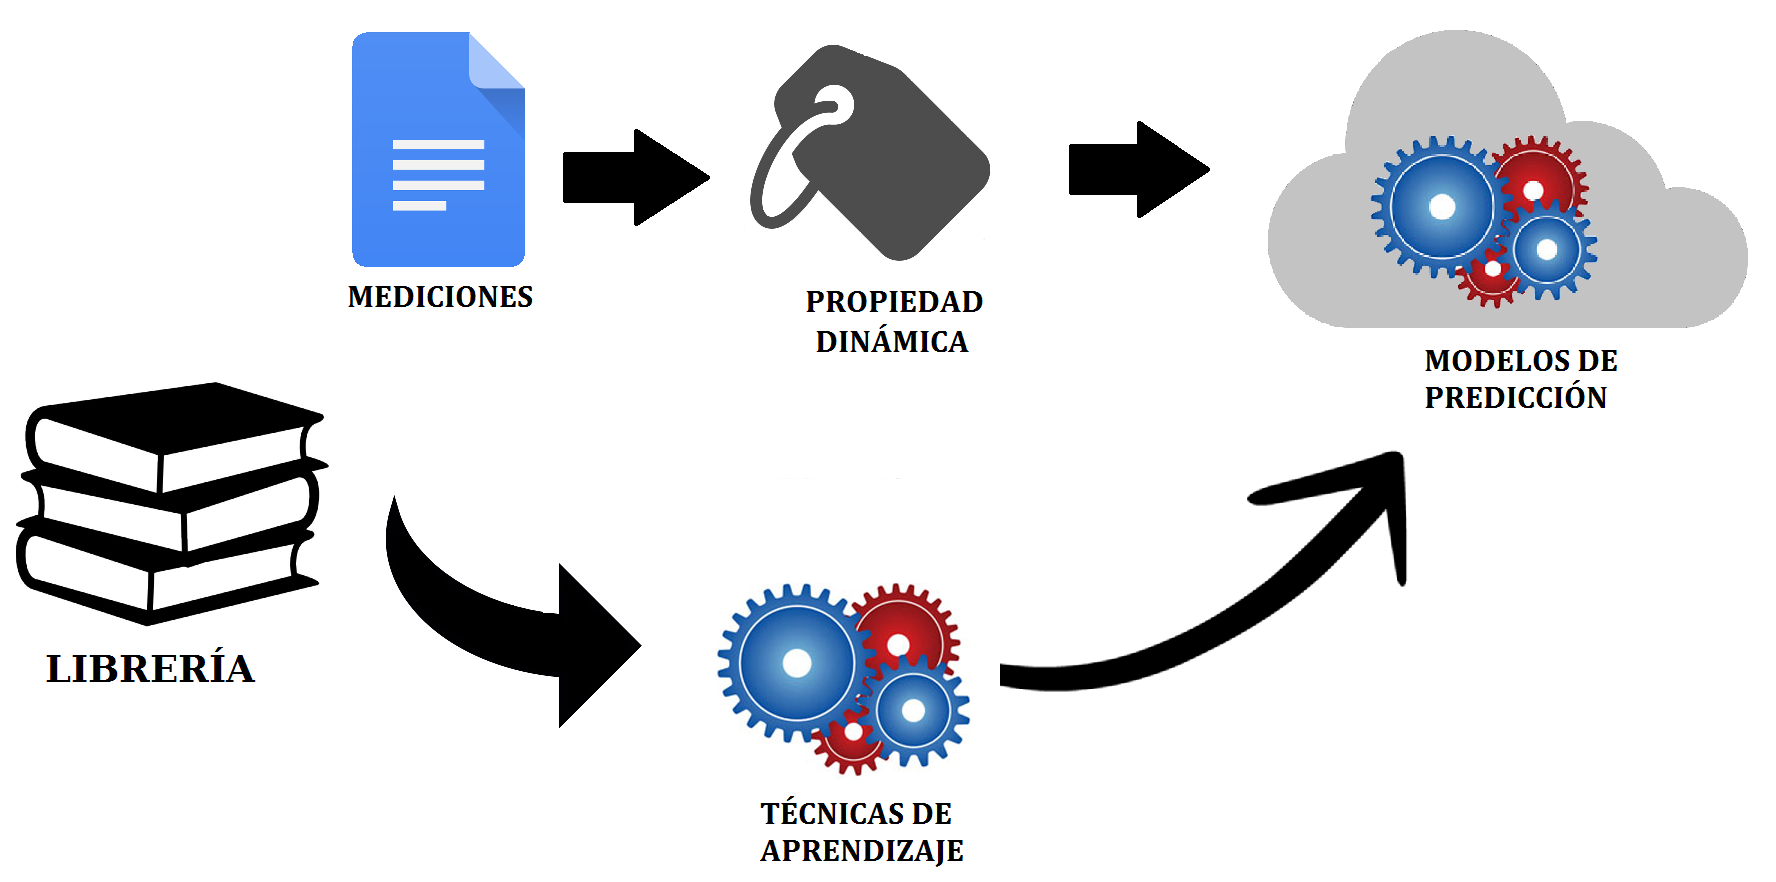
\includegraphics[scale=0.55]{C:/Users/usuario/Tesisworkspace/Tesis_Standalone/tesis/images/prediction-workflow}
\par\end{centering}

\caption{Diagrama de flujo del proceso de entrenamiento de modelos.\label{fig:prediction-workflow}}
\end{figure}


La selección de la librería de aprendizaje automático es el punto
de partida condicionando el resto de los datos configurables. Luego,
al seleccionar el archivo fuente con los benchmarks medidos en formato
CSV, a través de un proceso de parseo se obtiene el archivo comúnmente
llamado dataset adaptado al formato de instancias de la librería.
Con este nuevo formato se extraen los atributos para seleccionar aquel
que se pretenda predecir y junto con la selección de algoritmos se
inicia la optimización de los mismos. 

Los algoritmos de aprendizaje se habilitan al momento de elegir la
librería a utilizar ofreciendo sólo aquellos que la librería dispone.
La multi selección de clasificadores brinda la posibilidad al usuario
de elegir los algoritmos de mayor preferencia o interés para optimizar
en ese momento evitando el proceso de optimización de todos los clasificadores
lo cual significaría un ahorro en el uso de los recursos computacionales. 

Finalmente, como resultado de esta etapa se obtiene el conjunto de
clasificadores seleccionados cuyas configuraciones son las más favorables
para los datos de entrenamiento 


\subsubsection{Evaluación de modelos}

En esta sección se detallarán las consideraciones y los enfoques generales
del proceso de evaluación y métricas de error. También, se especificará
el flujo de las actividades llevadas a cabo para calificar el desempeño
del clasificador y realizar ajustes de ser necesario. 


\subsubsection*{Evaluación}

El dataset de origen, también denominado conjunto de datos de aprendizaje
o entrenamiento, es utilizado para obtener el modelo predictivo que
generalice esos datos adecuadamente. El término generalizar hace referencia
a obtener una función que se ajuste a los datos en cuanto minimice
el \emph{error empírico} que es el error producido por el algoritmo. 

El proceso de evaluación, entonces, debe utilizar nuevos datos de
entrada (preferentemente distintos al conjunto de entrenamiento) y
predecir la salida a partir de éstos arrojando ciertamente una tasa
de error en la predicción hecha por el clasificador. Existen dos métodos
clásicos de evaluación en base al origen de los datos usados para
la validación de modelos. El más sencillo resulta de utilizar los
mismos datos que fueron usados para la fase de entrenamiento. El método
restante conocido bajo el nombre de validación cruzada (\emph{Cross
validation}) tiene una metodología más compleja. 

El método de validación cruzada utiliza un coeficiente \emph{K} de
repetición y división; los datos de entrada se dividen en \emph{K}
subconjuntos, utilizando uno de ellos como dato de prueba y el resto
(\emph{K-1}) como datos de entrenamiento. El proceso es repetido durante
\emph{K} iteraciones, con cada uno de los posibles subconjunto de
datos de prueba. Finalmente se calcula la media aritmética de los
resultados de cada iteración para obtener un único resultado. Los
resultados de la evaluación son contemplan mediante un conjunto de
indicadores que se describirán más adelante. Nekonata implementa ambos
métodos e incluye la funcionalidad necesaria para acceder a todos
los valores predictivos. 


\subsubsection*{Métricas}

Las métricas usadas para la evaluación de los algoritmos simplemente
son fórmulas matemáticas o composición de ellas que involucran únicamente
a dos variables, los valores reales del dominio y los valores predictivos.
En la herramienta se ha implementado el conjunto de indicadores más
popular brindando, conjuntamente, la posibilidad de utilizar las métricas
ofrecidas por cada biblioteca incorporada. También, se han definido
e incorporado cuatro características globales asociadas a las métricas
para brindar soporte a otras funcionalidades. Toda métrica \emph{i})
brinda algún tipo de información, acerca del error de predicción o
estadísticas o atributos de los datos; \emph{ii}) tiene una representación
particular de los indicadores, los valores pueden estar normalizados
en una escala del 0 al 1, expresados en porcentajes o simplemente
adaptados a la escala de los datos; \emph{iii}) definen por su naturaleza
un requerimiento minimo o maximo de su indicador y \emph{iv}) son
aplicables a un tipo de función ya sea regresión o clasificación. 

Con el fin de extremar las mejoras y asegurar que el modelo resultante
sea el más favorable para el conjunto de datos usados en el entrenamiento
el proceso de evaluación de modelos fue dividido en dos fases. Luego
de la etapa de entrenamiento, los algoritmos clasificadores optimizados
son expuestos a una serie de métricas dispuestos de manera tal que
permita visualizar las diferencias de desempeño entre clasificadores
con la misma métrica considerada. Esta vista es un recurso ofrecido
al usuario para decidir aquel modelo que a su criterio tenga mejor
calidad a través de la comparación simultánea y continuar mejorando
el modelo elegido a partir del análisis de los efectos de underfit
y overfit. 


\subsubsection*{Fase 1: Comparación de modelos}

La optimización de un algoritmo clasificador para obtener la configuración
más apropiada para el conjunto de datos es conveniente,sin embargo,
resulta más útil aplicar un proceso de optimización a un conjunto
de algoritmos candidatos para luego analizar cuál de ellos es el que
mejor generaliza los datos. La comparación entre clasificadores se
realiza por medio de métricas que arrojan una estimación acerca del
error de predicción, es decir, una medida que refleja la diferencia
entre los datos reales del dominio y los valores predichos por el
algoritmo. Es conveniente trasladar el análisis a la mayor cantidad
de métricas posibles, ya que un mismo indicador podría arrojar valores
cercanos entre un algoritmo y otro favoreciendo equivocadamente a
uno de ellos, error que podría notarse al compararlos simultáneamente
con otras métricas. La metodología de operación de esta fase se muestra
en la figura \ref{fig:models-comparison-workflow}. 

Nekonata hace foco en este detalle y ofrece al usuario una vista de
imágenes con los indicadores medidos de cada algoritmo seleccionado
por el usuario para aplicar el proceso de optimización y elegir, posteriormente,
el que resulte más adecuado. La información gráfica complementaria
que se brinda, detalla los algoritmos representados por medio de barras
y agrupados en categorías separadas de acuerdo a cada métrica a modo
de facilitar la comparación. Adicionalmente las barras se colorean
en dos tonos diferentes para acentuar, por cada métrica, los clasificadores
que significarían las mejores opciones para ese indicador. 

\begin{figure}
\begin{centering}
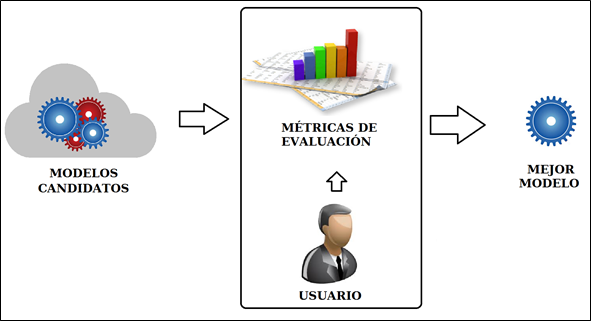
\includegraphics[scale=0.55]{C:/Users/usuario/Tesisworkspace/Tesis_Standalone/tesis/images/models-comparison-workflow}
\par\end{centering}

\caption{Diagrama de flujo de la fase de comparación de modelos. \label{fig:models-comparison-workflow}}
\end{figure}


La disposición de todas las métricas de evaluación se han distribuido
en imágenes dispares para agruparlas según la clase de información
que representan, ya sean indicadores del error de predicción o características
sobre los datos. En el primer caso también se distinguen entre aquellas
métricas interpretadas a valores normalizados entre cero y uno y métricas
a valores de escala del atributo. De esta forma se agrupan en conjuntos
los indicadores proclives a compararse mutuamente como puede observarse
en la figura \ref{fig:screenshot-errors}. 

El aporte del usuario se incorporó para personificar el interés y
criterio para determinar los indicadores más significativos para basar
la elección del modelo más favorable. De esta manera, cada usuario
puede basar su elección analizando y comparando los indicadores que
a su criterio son más relevantes. 

\begin{figure}
\begin{centering}
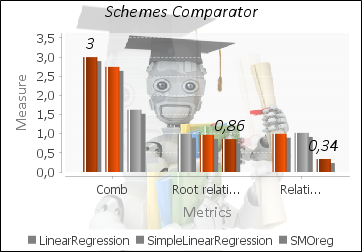
\includegraphics[scale=0.55]{C:/Users/usuario/Tesisworkspace/Tesis_Standalone/tesis/images/screenshot-errors}
\par\end{centering}

\caption{Captura de pantalla de la vista de indicadores sobre el error de predicción
normalizados.\label{fig:screenshot-errors}}
\end{figure}



\subsubsection*{Fase 2: Ajustes al modelo}

A través del uso de métricas se adquiere una idea estimativa del desempeño
del clasificador frente al conjunto de datos de entrenamiento, sin
embargo, podría resultar útil conocer el comportamiento general del
algoritmo, contrastando cada uno de los valores reales del atributo
clase con los valores predichos por el clasificador, y obtener así
una vista exacta de la manera en que el clasificador se ajusta a los
datos (Figura \ref{fig:screenshot-error-curve}). 

Este recurso es usado en la herramienta como un gráfico de dos líneas
continuas de distinto color para representar el conjunto de datos
de entrenamiento y el conjunto de datos predichos. Cada punto del
dominio corresponde a cada instancia y la unión entre puntos sólo
se realiza con fines ilustrativos. 

\begin{figure}
\begin{centering}
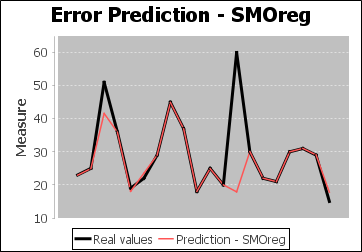
\includegraphics[scale=0.55]{C:/Users/usuario/Tesisworkspace/Tesis_Standalone/tesis/images/screenshot-error-curve}
\par\end{centering}

\caption{Captura de pantalla de la vista del error de predicción. \label{fig:screenshot-error-curve}}
\end{figure}


El análisis del error de predicción es la base para comprender la
calidad del modelo construido hasta el momento aunque no es el único
objetivo, ya que la vista permite extraer conocimiento de cómo se
comporta el conjunto de datos de entrenamiento, existencia de valores
extremos, la variación de los valores tomados, entre otros. Es un
recurso gráfico para complementar la información que se le brinda
al usuario y encaminarlo a un correcto proceso de ajuste del modelo. 

\begin{figure}
\begin{centering}
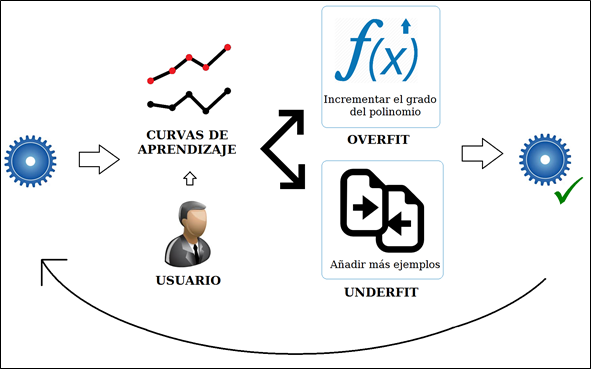
\includegraphics[scale=0.55]{C:/Users/usuario/Tesisworkspace/Tesis_Standalone/tesis/images/adjustment-workflow}
\par\end{centering}

\caption{Diagrama de flujo de la fase de ajuste.\label{fig:adjustment-workflow}}
\end{figure}


El flujo de desarrollo de esta fase se planteó como un proceso de
carácter opcional e iterativo para el usuario. Se puede optar simplemente
por almacenar el modelo elegido durante la etapa de comparación anterior
o repetir las veces que se desee un procedimiento de análisis de las
curvas de aprendizaje del modelo y las acciones consecuentes para
reparar los posibles efectos, como se muestra en la figura \ref{fig:adjustment-workflow}.


A continuación se explicará el funcionamiento de la fase brindando
una visión general del planteamiento de las curvas de aprendizaje
con las respectivas consideraciones que se tuvieron en cuenta y la
manera en que se ha incluido la participación del usuario para la
transformación del conjunto de datos. 


\paragraph*{Curvas de aprendizaje}

Las curvas de aprendizaje se componen por dos líneas de puntos representadas
en el mismo plano cartesiano. Ambas líneas grafican el error de predicción
utilizando los dos métodos de evaluación conocidos, aplicando el conjunto
de entrenamiento o el método de validación cruzada.Las curvas de aprendizaje
implementadas por la herramienta son mostradas en la figura \ref{fig:learning-curves}

El procedimiento considera una cantidad de instancias determinadas,
cantidad que se incrementa en un factor constante para aplicar el
modelo y calcular el error cuadrático medio, es decir, la diferencia
cuadrática entre el valor real del atributo y el predicho por el modelo. 

En un primer paso, la herramienta toma en cuenta las primeras cinco
instancias, luego las primeras diez, las primeras quince y así sucesivamente
para conformar cada punto del dominio cuyo valor de ordenada es el
error cuadrático, error añadido en la herramienta como parte del conjunto
de métricas consideradas. Por cuestiones de facilitar la vista se
impuso un límite en los valores del dominio reducido en trescientas
(300) instancias en caso de que el conjunto de entrenamiento supere
dicha cantidad. 




\paragraph*{Opciones para el usuario}

En Nekonata se han incluido dos acciones posibles para reparar, en
caso de evidenciar, los efectos de overfit o underfit del modelo.
Estas dos acciones no son mutuamente excluyentes de manera que el
usuario puede elegir libremente alguna o ambas acciones a la vez,
sin embargo, la herramienta le recomienda la acción que debería tomar
en caso de un efecto u otro. Ambas acciones realizan una transformación
en la base de datos, cuando el usuario decide incorporar nuevas instancias
o ejemplos del dominio introduce un archivo el cuál es parseado al
formato conocido por la librería de uso y es unido al conjunto original
siendo ahora, el nuevo conjunto de datos. Por otro lado, cuando el
usuario decide aumentar el grado del polinomio que emplea el modelo,
elige un número entre uno y cuatro para modificar este polinomio y
así, añadir a la base de datos los nuevos atributos originarios del
nuevo polinomio completo para ese grado. 


\subsubsection{Diseño e implementación}

A pesar que la herramienta fue pensada para la predicción de componentes
de android,se desarrolló como una aplicación de escritorio debido
a la limitación del hardware de los dispositivos móviles para ejecutar
los procesos de optimización que consumen un gran porcentaje de recursos
computacionales. Esta implementación desvincula la herramienta de
medición con la herramienta de entrenamiento y evaluación de modelos,
permitiendo la ejecución independiente entre ambas por lo que el puente
de comunicación entre ellas es la correspondencia entre la salida
de la primer herramienta con la entrada de la segunda; la herramienta
de medición crea archivos de formato \ac{CSV}, los cuales serán usados
en la herramienta como el conjunto de datos fuente para el entrenamiento. 


\subsubsection*{Entorno y tecnologías}

Para la implementación del framework Nekonata se utilizó el entorno
de desarrollo Eclipse cuyo lenguaje de programación es Java. El proyecto
ha sido configurado con la versión \ac{JDK} 1.7 y \ac{JRE} 1.8 y
además, se han incorporado tecnologías de terceros para el entorno
las cuáles cumplen distintos roles en la herramienta. 

Para el diseño de la interfaz gráfica se utilizó mayormente la librería
SWING de java incorporada en el \ac{JDK} aunque también se incluyeron
componentes de la librería nativa AWT. La principal ventaja de la
librería SWING es brindar una interfaz adaptada a cada sistema operativo
sin necesidad de cambio de código, es decir independiente a la plataforma.
Complementariamente se incorporaron las dos siguientes librerías:
\emph{jgoodies-forms-1.8.0.jar} y \emph{miglayout15-swing.jar}

Por otro lado, para la creación de vistas para el usuario se incorporó
la biblioteca gráfica de Java JFREECHART que facilita la creación
de varios tipos de gráficos profesionales, en el caso de la herramienta
se han utilizado los gráficos de barras y lineales para representar
la información requerida por el usuario. Esta biblioteca ha sido elegida
por brindar objetos de alta calidad y ofrecer una extensa gama de
funciones para reforzar y mejorar la información mostrada en los gráficos.
Se utilizó la versión 1.0.19 de la biblioteca en complemento con la
librería JCOMMON en la versión 1.0.23. 

Respecto al uso de técnicas de aprendizaje de máquina, actualmente
existen muchas tecnologías y frameworks que proveen esta funcionalidad
para utilizar en entornos Java, sin embargo, como se ha adelantado
anteriormente en la herramienta sólo se incluyó la biblioteca \emph{Weka}
en la versión 3.8 y se añadió también un paquete para la optimización
de parámetros perteneciente a la misma librería denominado MULTISEARCH
en su versión más actual del mes de agosto del 2016. 


\subsubsection*{Diseño}

Considerando todo lo anteriormente descrito, el concepto principal
de la herramienta fue la extensibilidad de la misma desde todos los
enfoques posibles. Esto significa que la herramienta pudiera aceptar
diferentes tipos de librerías de aprendizaje de máquina, datasets,
modelos de regresión, parámetros y métricas; lo que conlleva a un
gran grado de abstracción de las clases que conforman la aplicación
y, por lo tanto, se consideró importante la asociación de mismas,
para un entendimiento mayor de parte de un nuevo desarrollador.

La finalidad de la etapa de implementación fue un buen framework de
trabajo para el futuro desarrollo de modelos, librerías y métricas.
Si bien la herramienta sólo trabaja con Weka actualmente y la mayoría
de su funcionalidad es enteramente parser , se considera que el grado
de abstracción es lo bastante elevado para poder soportar la finalidad
deseada.

Aplicando los conceptos teóricos antes presentados, se exponen a continuación
los paquetes y las clases principales que componen el desarrollo de
Nekonata. 


\paragraph*{Databases}

Como ya se mencionó anteriormente se desea poder administrar, leer
y escribir datasets de forma dinámica y segura. Para esto, se creó
una estructura para almacenar cada individuo (instancia) con una estructura
\emph{Hashtable}, con los nombres de los atributos como claves de
los valores numéricos que representan a cada uno de ellos.

Asimismo, se desarrolló un conjunto para representar los datasets
ya que son estos las bases de los modelos, del aprendizaje y del framework,
tomando como entrada un csv y creando la base de datos necesaria para
el correcto funcionamiento de la aplicación. 

\begin{figure}
\begin{centering}
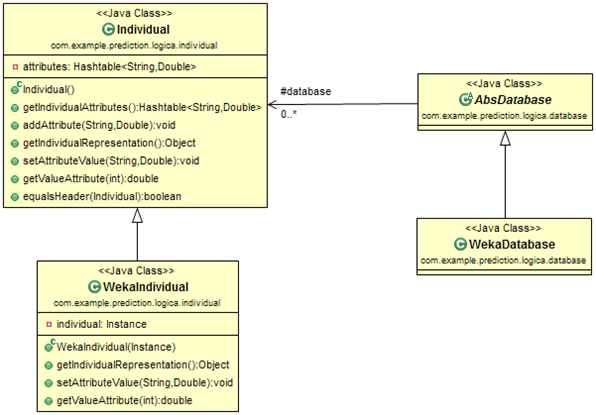
\includegraphics[scale=0.55]{C:/Users/usuario/Tesisworkspace/Tesis_Standalone/tesis/images/database-class-diagram}
\par\end{centering}

\caption{Diagrama de clases de las bases de datos implementadas\label{fig:database-class-diagram}}
\end{figure}



\paragraph*{Modelos}

Los modelos que la herramienta presenta son de tipo regresivo pero
no necesariamente son modelos intrínsecamente predictivos y por eso
el framework presenta una división clara entre modelos regresivos
y clasificadores (siempre considerando que estos últimos se utilizan
para la regresión).

\begin{figure}
\begin{centering}
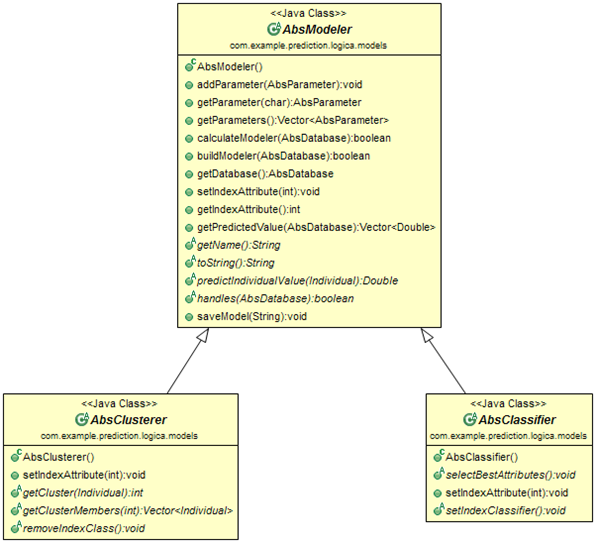
\includegraphics[scale=0.55]{C:/Users/usuario/Tesisworkspace/Tesis_Standalone/tesis/images/modelers-class-diagram}
\par\end{centering}

\caption{Diagrama de clases de los modelos base implementados.\label{fig:modelers-class-diagram}}
\end{figure}


A partir de esto, implementando los métodos abstractos presentados,
se pueden incluir cualquier método de clasificación requerido, siempre
considerando importante que retorne un valor denso. Actualmente, los
modelos implementados son los presentados en la sección \ref{subsec:Funciones-contempladas}.

\begin{figure}
\begin{centering}
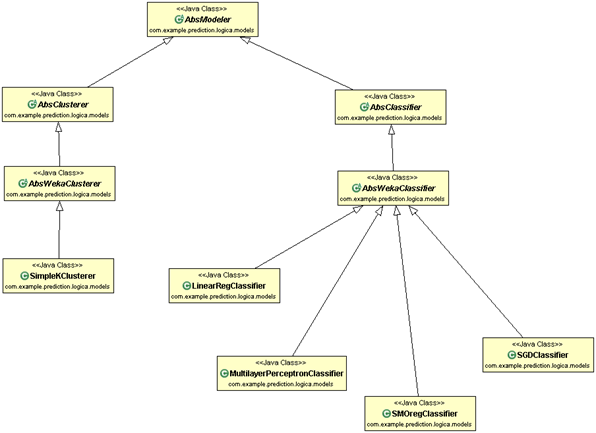
\includegraphics[scale=0.55]{C:/Users/usuario/Tesisworkspace/Tesis_Standalone/tesis/images/all-modelers-class-diagram}
\par\end{centering}

\caption{Diagrama de la relación entre los modelos implementados.\label{fig:all-modelers-class-diagram}}
\end{figure}


Como se puede apreciar en la figura \ref{fig:all-modelers-class-diagram}
, se realizó una abstracción intermedia considerando la librería Weka.
Esto se debe principalmente al comportamiento en común que tenían
dichos modelos, pero no es mandatoria dicha abstracción al agregar
una nueva librería o al agregar nuevos modelos. 

Ya que el diseño fue impulsado por la necesidad de abstracción e independencia
de las librerías subyacentes, se considera importante la posibilidad
de que en un futuro cualquier desarrollador pueda incorporar modelos
implementados de forma particular. 


\paragraph{Parámetros}

Para implementar los modelos, la iniciativa fue modelar el concepto
teórico que los rige: funciones. Como ya fue explicado, las funciones
están moldeados por variables y parámetros. Las variables son aquellos
atributos modelados por la Hashtable en la clase individuo. Debido
a los modelos considerados en el apartado anterior, los parámetros
(o las constantes de una función) fueron modeladas en dos partes:
\begin{enumerate}
\item Parámetros simples: Son aquellos que sólo tienen un valor numérico
y que tiene un valor único en la función. Rigen en funcionamiento
del método de aprendizaje y determinan la calidad y finalidad que
tendrán los mismos. Estos tipos de parametros se utilizan en todo
el core de modelos ya que son la idea fundamental de cualquier función
matemática. 
\item Parámetros kernel: Son funciones matemáticas que se emplean en las
\ac{SVM}. Estas funciones son las que le permiten convertir lo que
sería un problema de clasificación no lineal en el espacio dimensional
original, a un sencillo problema de clasificación lineal en un espacio
dimensional mayor. Debido a que estas son funciones dentro de los
modelos, es conveniente el modelado de las mismas de forma particular.
\end{enumerate}
Observando ambos puntos, se puede apreciar una composición de parámetros
ya que las funciones se conforman por parámetros simples y los parámetros
kernel son funciones internas. Esto se puede observar en la figura
\ref{fig:parameters-class-diagram} . 

\begin{figure}
\begin{centering}
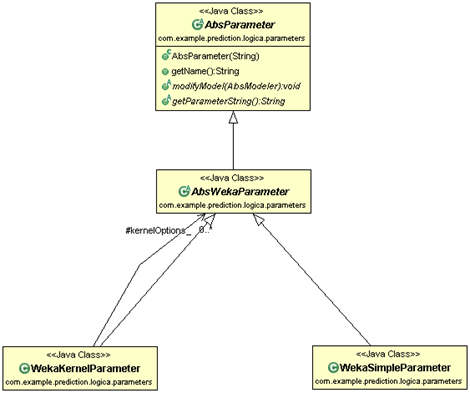
\includegraphics[scale=0.55]{C:/Users/usuario/Tesisworkspace/Tesis_Standalone/tesis/images/parameters-class-diagram}
\par\end{centering}

\caption{Diagrama de clases de los parametros implementados\label{fig:parameters-class-diagram}}
\end{figure}



\paragraph{Métricas}

Otra parte importante de la implementación de la herramienta es la
capacidad de la misma de cuantificar y valorizar los modelos obtenidos.
Las mismas ya vienen implementadas por la librería Weka, pero considerando
la finalidad de abstraer comportamiento, las mismas fueron parseadas
y se crearon nuevas clases.

\begin{figure}
\begin{centering}
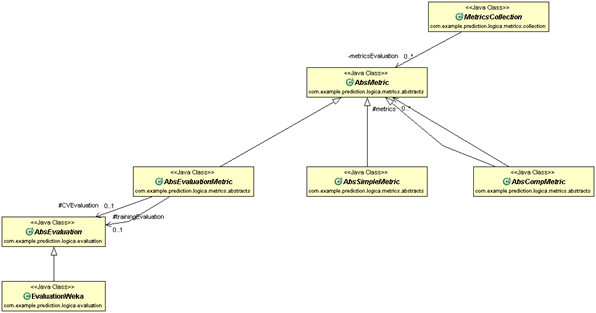
\includegraphics[scale=0.55]{C:/Users/usuario/Tesisworkspace/Tesis_Standalone/tesis/images/metrics-class-diagram}
\par\end{centering}

\caption{Diagrama de clases de las métricas implementadas.\label{fig:metrics-class-diagram}}
\end{figure}


La implementación presentada surge a partir de la forma de implementación
que tiene la librería weka. La misma presenta una clase que representa
la relación entre los valores reales que presenta la base de datos
y los valores calculados por el modelo. Sin embargo, la librería presenta
la particularidad de solo calcular métricas de los modelos que la
misma toma como de regresión. Así, el Simple K clusterer quedaría
excluido de este grupo y, por lo tanto, no podría ser valorado. La
implementación planteada permite que este modelo quede a la altura
de los otros presentados y que, si se desea, se pueden crear nuevas
métricas sin tener la clase \emph{AbsEvaluation} que represente esta
relación. Sólo sería necesario crear la métrica heredando de \emph{AbsSimpleMetric}
e implementar la forma de cálculo requerida.


\paragraph*{Optimización}

El paquete que se procede a explicar es implementado principalmente
considerando la función que proviene de Weka, permitiendo la prueba
de varios valores para los parámetros sin necesidad de pruebas constantes,
apuntando a una mejor y más rápida optimización del modelo. Puede
omitirse dicha implementación si se desea agregar un nuevo modelo,
pero es conveniente la explicación del mismo para futuras adaptaciones
de modelos de weka que se quieran agregar o de librerías que tengan
esta posibilidad también. 

La idea del paquete de optimización es que, de forma transparente
para el usuario de la aplicación, el modelo consiga adaptarse a la
base de datos analizada. Esto permite que la aplicación Nekonata pueda
adaptarse a grandes rangos de valores objetivo. Como ya se dijo anteriormente,
no es un paquete necesario en la aplicación ya que los parámetros
pueden ser puestos de forma fija en un modelo, pero esto restringe
el rango y las posibilidades del mismo. 

Los optimizadores cumplen la función de probar valores para los parámetros
y se quedan con aquellos que minimizan el grado de error del modelo.
Asimismo, cabe destacar que Weka proporciona dos tipos de optimizadores.
Los primeros son los simples, que consideran cada parámetro del modelo
desde un valor al otro. Los segundos son los kernels y prueban valores
no solo para los parámetros propios de los modelos sino para los parámetros
que conforman los kernels. 

\begin{figure}
\begin{centering}
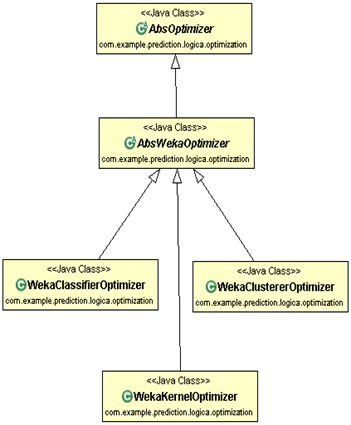
\includegraphics[scale=0.55]{C:/Users/usuario/Tesisworkspace/Tesis_Standalone/tesis/images/optimizer-class-diagram}
\par\end{centering}

\caption{Diagrama de clases de los optimizadores implementados.\label{fig:optimizer-class-diagram}}
\end{figure}



\paragraph*{Cómo agregar clases nuevas}

Todo lo anteriormente planteado se mantiene coherente y de forma congruente
gracias a la clase librería y lo que conlleva agregarla a la aplicación. 

\begin{figure}
\begin{centering}
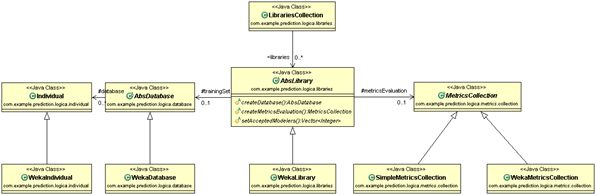
\includegraphics[scale=0.55]{C:/Users/usuario/Tesisworkspace/Tesis_Standalone/tesis/images/library-class-diagram}
\par\end{centering}

\caption{Diagrama de clases de las librerias y las relaciones con los otros
objetos.\label{fig:library-class-diagram}}
\end{figure}


Al crear la librería, y como se ve en el diagrama de clases, se deben
implementar dos métodos que devuelven dos conceptos principales. Por
un lado, un objeto de tipo Database que ya se explicó anteriormente.
Por el otro, un objeto MetricsCollection. Este último representa el
conjunto de métricas que sirven para valorizar los modelos. 

Ya implementado se provee el conjunto \emph{SimpleMetricsCollection}
que permiten valorizar cualquier modelo, ademas del \emph{WekaMetricsCollection}
que sólo contiene la metricas basadas en el \emph{WekaEvaluation}. 

La última función que se debe implementar de forma ineludible retorna
un vector de constantes. Estas constantes deben estar declaradas en
la clase \emph{Config.Modeler} con el formato: 

\fbox{\begin{minipage}[t]{1\columnwidth}%
\begin{center}
Nombre a mostrar en la aplicación: constante 
\par\end{center}%
\end{minipage}}

Las mismas declaran los modelos que son aceptados por la liberia.
Esto se hace a modo de índice para los modelos y, al momento de utilizar
la herramienta, las clases de los modelos sean creadas al momento
de ser seleccionadas. Esto se permite implementando la última función: 

\lstinline[language=Java,basicstyle={\footnotesize}]!public abstract Vector<AbsModeler> createModelers(Vector<Integer> selectedModels, int index);!

Esta última función crea la relación entre la constante con las clases
que se deben crear para representar a los modelos. 

\begin{figure}
\begin{centering}
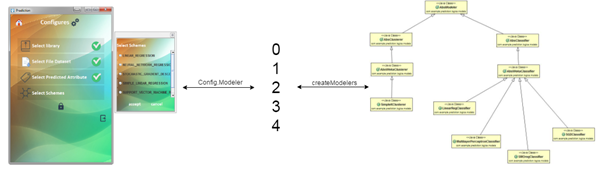
\includegraphics[scale=0.55]{C:/Users/usuario/Tesisworkspace/Tesis_Standalone/tesis/images/config-correlation}
\par\end{centering}

\caption{Diagrama conceptual de la configuración que presenta la herramienta\label{fig:config-correlation}}
\end{figure}



\subsubsection{Formato de los resultados\label{subsec:Formato-de-los}}

La herramienta devuelve como resultado un archivo en formato TXT almacenando,
por un lado, los valores resultantes de los parámetros fundamentales
de cada técnica y, por otro lado, la descripción del modelo construido.
La herramienta genera un archivo por cada técnica elegida por el usuario
para optimizar, en la dirección especificada en la configuración bajo
el nombre de la técnica. La figura \ref{fig:linear-regression-result}
permite una descripción gráfica de lo expresado anteriormente, donde
detalla A) los parámetros, B) Nombre del modelo y C) la función definida
para el atributo de predicción. 

\begin{figure}[H]
\begin{centering}
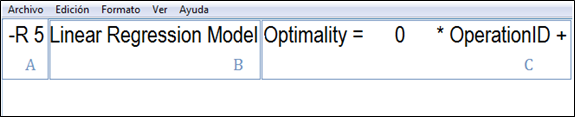
\includegraphics[scale=0.55]{C:/Users/usuario/Tesisworkspace/Tesis_Standalone/tesis/images/linear-regression-result}
\par\end{centering}

\caption{Ejemplo de resultado del modelo ‘Linear Regression’. \label{fig:linear-regression-result}}
\end{figure}


La manera en que los datos son expuestos al usuario no representa
un formato compatible para cualquier herramienta sobre aprendizaje
de máquina, esto se debe a que no existe actualmente, un formato estándar
para almacenar los modelos, y esta discrepancia entre las herramientas
disponibles exige un seteo manual de las técnicas por cada evaluación
que se realice
